% MIT License

% Copyright (c) 2022 Chiyuru

% Permission is hereby granted, free of charge, to any person obtaining a copy of this software and associated documentation files (the "Software"), 
% to deal in the Software without restriction, including without limitation the rights
% to use, copy, modify, merge, publish, distribute, sublicense, and/or sell
% copies of the Software, and to permit persons to whom the Software is
% furnished to do so, subject to the following conditions:

% The above copyright notice and this permission notice shall be included in all copies or substantial portions of the Software.

% THE SOFTWARE IS PROVIDED "AS IS", WITHOUT WARRANTY OF ANY KIND, EXPRESS OR IMPLIED, INCLUDING BUT NOT LIMITED TO THE WARRANTIES OF MERCHANTABILITY,
% FITNESS FOR A PARTICULAR PURPOSE AND NONINFRINGEMENT. IN NO EVENT SHALL THE AUTHORS OR COPYRIGHT HOLDERS BE LIABLE FOR ANY CLAIM, DAMAGES OR OTHER
% LIABILITY, WHETHER IN AN ACTION OF CONTRACT, TORT OR OTHERWISE, ARISING FROM,
% OUT OF OR IN CONNECTION WITH THE SOFTWARE OR THE USE OR OTHER DEALINGS IN THE SOFTWARE.

\documentclass[UTF8]{ctexart}

\usepackage{amsmath}
\usepackage{cases}
\usepackage{cite}
\usepackage{graphicx}
\usepackage[margin=1in]{geometry}
\usepackage{float}
\geometry{a4paper}
\usepackage{fancyhdr}
\usepackage{multirow}
\usepackage{listings}
\pagestyle{fancy}
\fancyhf{}


\title{ICS-lab2实验报告}
\author{孔浩宇 PB20000113}
\date{\today}
\pagenumbering{arabic}

\begin{document}

\fancyhead[L]{孔浩宇}
\fancyhead[C]{ICS-lab2实验报告}
\fancyfoot[C]{\thepage}

\maketitle
\tableofcontents
\newpage

\section{实验目的}
    使用LC-3汇编语言求类斐波那契数列第$N$项$F(N)$.其中
    \[
        F(0) = F(1) = 1
    \]
    \[
        F(N) = F(N-2)\% p + F(N-1)\% q \ (2\leq N\leq 1024)
    \]
    \[
        p=2^k\ (2\leq k\leq 10),\ 10\leq q\leq 1024
    \]

\section{实验原理}
    \subsection{数列递推}
    在计算$F(N)$时,不妨用$R_i$保存$F(N-2)$,$R_j$保存$F(N-1)$,令
    \[
        R_m = F(N-2)\%p ,\ R_n = F(N-1)\%q  
    \]
    则
    \[
        F(N) = R_m + R_n.
    \]
    此时令
    \[
        R_i = R_j = F(N-1) , R_j = F(N).
    \]
    \subsection{二进制数取余}
        \subsubsection{$R_j \% q$}
        利用以下算法
        \begin{enumerate}
            \item [(1)]令$R_j = R_j - q$,若$R_j < 0 $,转$(2)$,否则转$(1)$.
            \item [(2)]令$R_j = R_j + q$,此时$R_j$即为所求,算法结束.
        \end{enumerate}
        设$R_j = J$不难看出在求$R_n \% q$的过程中,时间花费为$1+ J/q$.
        
        \subsubsection{$R_i \% p$}
        设$R_i = I[15:0]$,由$p=2^k$可得
        \[
            R_i \% p = I[k-2:0],\ \mbox{即}
            R_i \% p = I \& (p-1)
        \]

    \subsection{循环终止条件}
    利用寄存器$R_k$来判断当前$R_j$存储的数列下标.初始状态$R_k=N,\ R_j=F(0)=1,\ R_i=0$.
    \begin{enumerate}
        \item [(0)]$R_k = R_k - 1$,若为负,则转$(5)$ 
        \item [(1)]进行一次递推算法
        \item [(2)]转$(0)$
        \item [(3)]循环终止,输出$R_j$即为所求$F(N)$.
    \end{enumerate}

\section{实验步骤}
\subsection{初始化}
\begin{enumerate}
    \item [(0)]标号
    \begin{lstlisting}[basicstyle=\ttfamily,language={[x86masm]Assembler}]
        P       .FILL x3100         ;p
        Q       .FILL x3101         ;q
        N       .FILL x3102         ;N
        S       .FILL x3103         ;F(N)
    \end{lstlisting}

    \item [(1)]读入$p,q,N$
    \begin{lstlisting}[basicstyle=\ttfamily,language={[x86masm]Assembler}]
        .ORIG   x3000
            LDI R0, P           ; R0=P
            LDI R1, Q           ; R1=Q
            LDI R2, N           ; R2=N
    \end{lstlisting}

    \item [(2)]初始化其他变量
    \begin{lstlisting}[basicstyle=\ttfamily,language={[x86masm]Assembler}]
        ADD R0, R0, #-1         ; R AND R0 = R % P
        ADD R3, R3, #1          ; R3 <= F(N)
        AND R4, R4, #0          ; R4 <= F(N-1)
        NOT R7, R1          
        ADD R7, R7, #1          ; R + R7 = R - Q
    \end{lstlisting}
\end{enumerate}

\subsection{循环}
\begin{lstlisting}[basicstyle=\ttfamily,language={[x86masm]Assembler}]
    AGAIN   ADD R2, R2, #-1     ;
            BRn END             ; now the program end
            ADD R5, R4, #0      ; R5 = R4  F(N-2)
            ADD R6, R3, #0      ; R4 = R3  F(N-1)
            AND R5, R5, R0      ; R5 = F(N-2) % P
    BE      ADD R6, R6, R7      ; R6 = R6 - Q
            BRzp BE             ; Re
            ADD R6, R6, R1      ; R6 = F(N-1) % Q
            ADD R4, R3, #0      ; R4 = F(N-1)
            ADD R3, R5, R6      ; R3 = R4 + R5  F(N)
            BRnzp AGAIN         ; jump to AGAIN
\end{lstlisting}


\subsection{储存结果}
\begin{lstlisting}[basicstyle=\ttfamily,language={[x86masm]Assembler}]
    END     STI R3, S           ; store result
\end{lstlisting}

\subsection{结束}  
\begin{lstlisting}[basicstyle=\ttfamily,language={[x86masm]Assembler}]
    HALT.
\end{lstlisting}

\subsection{代码}    
\begin{lstlisting}[basicstyle=\ttfamily,language={[x86masm]Assembler}]
    .ORIG   x3000
        LDI R0, P           ; R0=P
        LDI R1, Q           ; R1=Q
        LDI R2, N           ; R2=N
        ADD R0, R0, #-1     ; now R & R0 = R mod P
        ADD R3, R3, #1      ; R3 is the result  F(N)
        AND R4, R4, #0      ; R4 is F(N-1)
        NOT R7, R1          
        ADD R7, R7, #1      ; now R + R7 = R - Q
        ; Initial
    
AGAIN   ADD R2, R2, #-1     ;
        BRn END             ; now the program end
        ADD R5, R4, #0      ; R5 = R4  F(N-2)
        ADD R6, R3, #0      ; R6 = R3  F(N-1)
        AND R5, R5, R0      ; R5 = F(N-2) % P
BE      ADD R6, R6, R7      ; R6 = R6 - Q
        BRzp BE             ; Re
        ADD R6, R6, R1      ; R6 = F(N-1) % Q
        ADD R4, R3, #0      ; R4 = F(N-1)
        ADD R3, R5, R6      ; R3 = R4 + R5  F(N)
        BRnzp AGAIN         ; jump to AGAIN
END     STI R3, S           ; store result
        HALT
P       .FILL x3100
Q       .FILL x3101
N       .FILL x3102
S       .FILL x3103
.END
\end{lstlisting}

\clearpage
\section{实验结果}
\begin{figure*}[htbp]
    \centering
    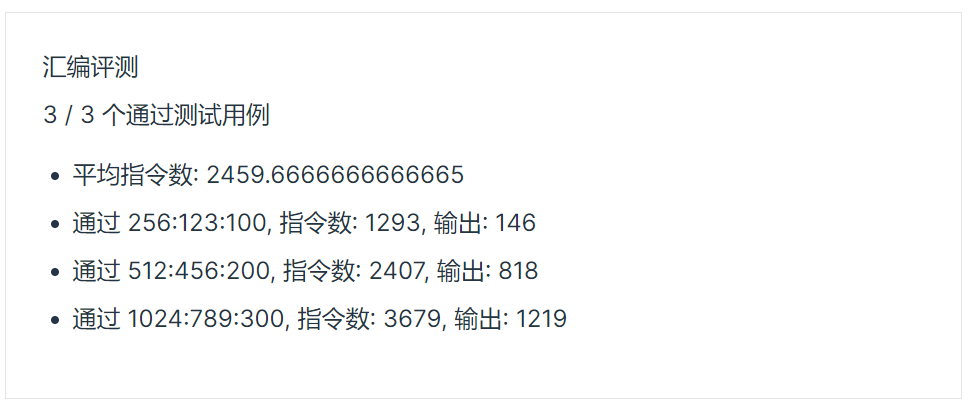
\includegraphics[scale=0.8]{re.png}
\end{figure*}

\section{实验改进}
将$F(N-2)$与$F(N-2)\% p$的存储寄存器改为一个,即$R_4 <= R_4 \% q = F(N-2) \% q$,
先利用$R_5$存储$F(N-1)$,即$R_5 <= R_3$,
再将$F(N-1)$与$F(N-1)\% p$的存储寄存器改为一个,即$R_3 <= R_3 \% p = F(N-1) \% q$,
之后令$R_3 <= R_3 + R_4 = F(N)$,再令$R_4 <= R_5 = F(N-1)$,一样可以完成循环,且节省一个寄存器.

利用节省下的寄存器改进$R_j \% q$的循环过程,令$R_6 = -2 q$ ,改进算法为
\begin{enumerate}
    \item [(1)]令$R_j = R_j - 2q$,若$R_j < 0 $,转$(2)$,否则转$(1)$.
    \item [(2)]令$R_j = R_j + q$,若$R_j >= 0 $,转$(3)$,否则转$(2)$.
    \item [(3)]此时$R_j$即为所求,算法结束.
\end{enumerate}
设$R_j = J$,在改进后的求$R_n \% q$的过程中,时间花费至多为$2 + J/2q$,当$J$较大时可大幅减少花费指令数.


\end{document}
\begin{lstlisting}[basicstyle=\ttfamily,language={[x86masm]Assembler}]
    
\end{lstlisting}